\chapter{Exemplo de anexo}

%=====================================================

Os apêndices são uma extensão do texto, destacados deste para evitar descontinuidade na sequência lógica ou alongamento excessivo de determinado assunto ou tópico secundário dentro dos capítulos da dissertação ou da tese. São contribuições que servem para esclarecer, complementar, provar ou confirmar as ideias apresentadas no texto dos capítulos e que são importantes para a compreensão dos mesmos.

Todos os apêndices devem vir após as referências bibliográficas e devem ser enumerados por letras maiúsculas (A, B, C, ...).

%=====================================================


Diagramas de caso de USO
\begin{figure}[!htb]
\centering
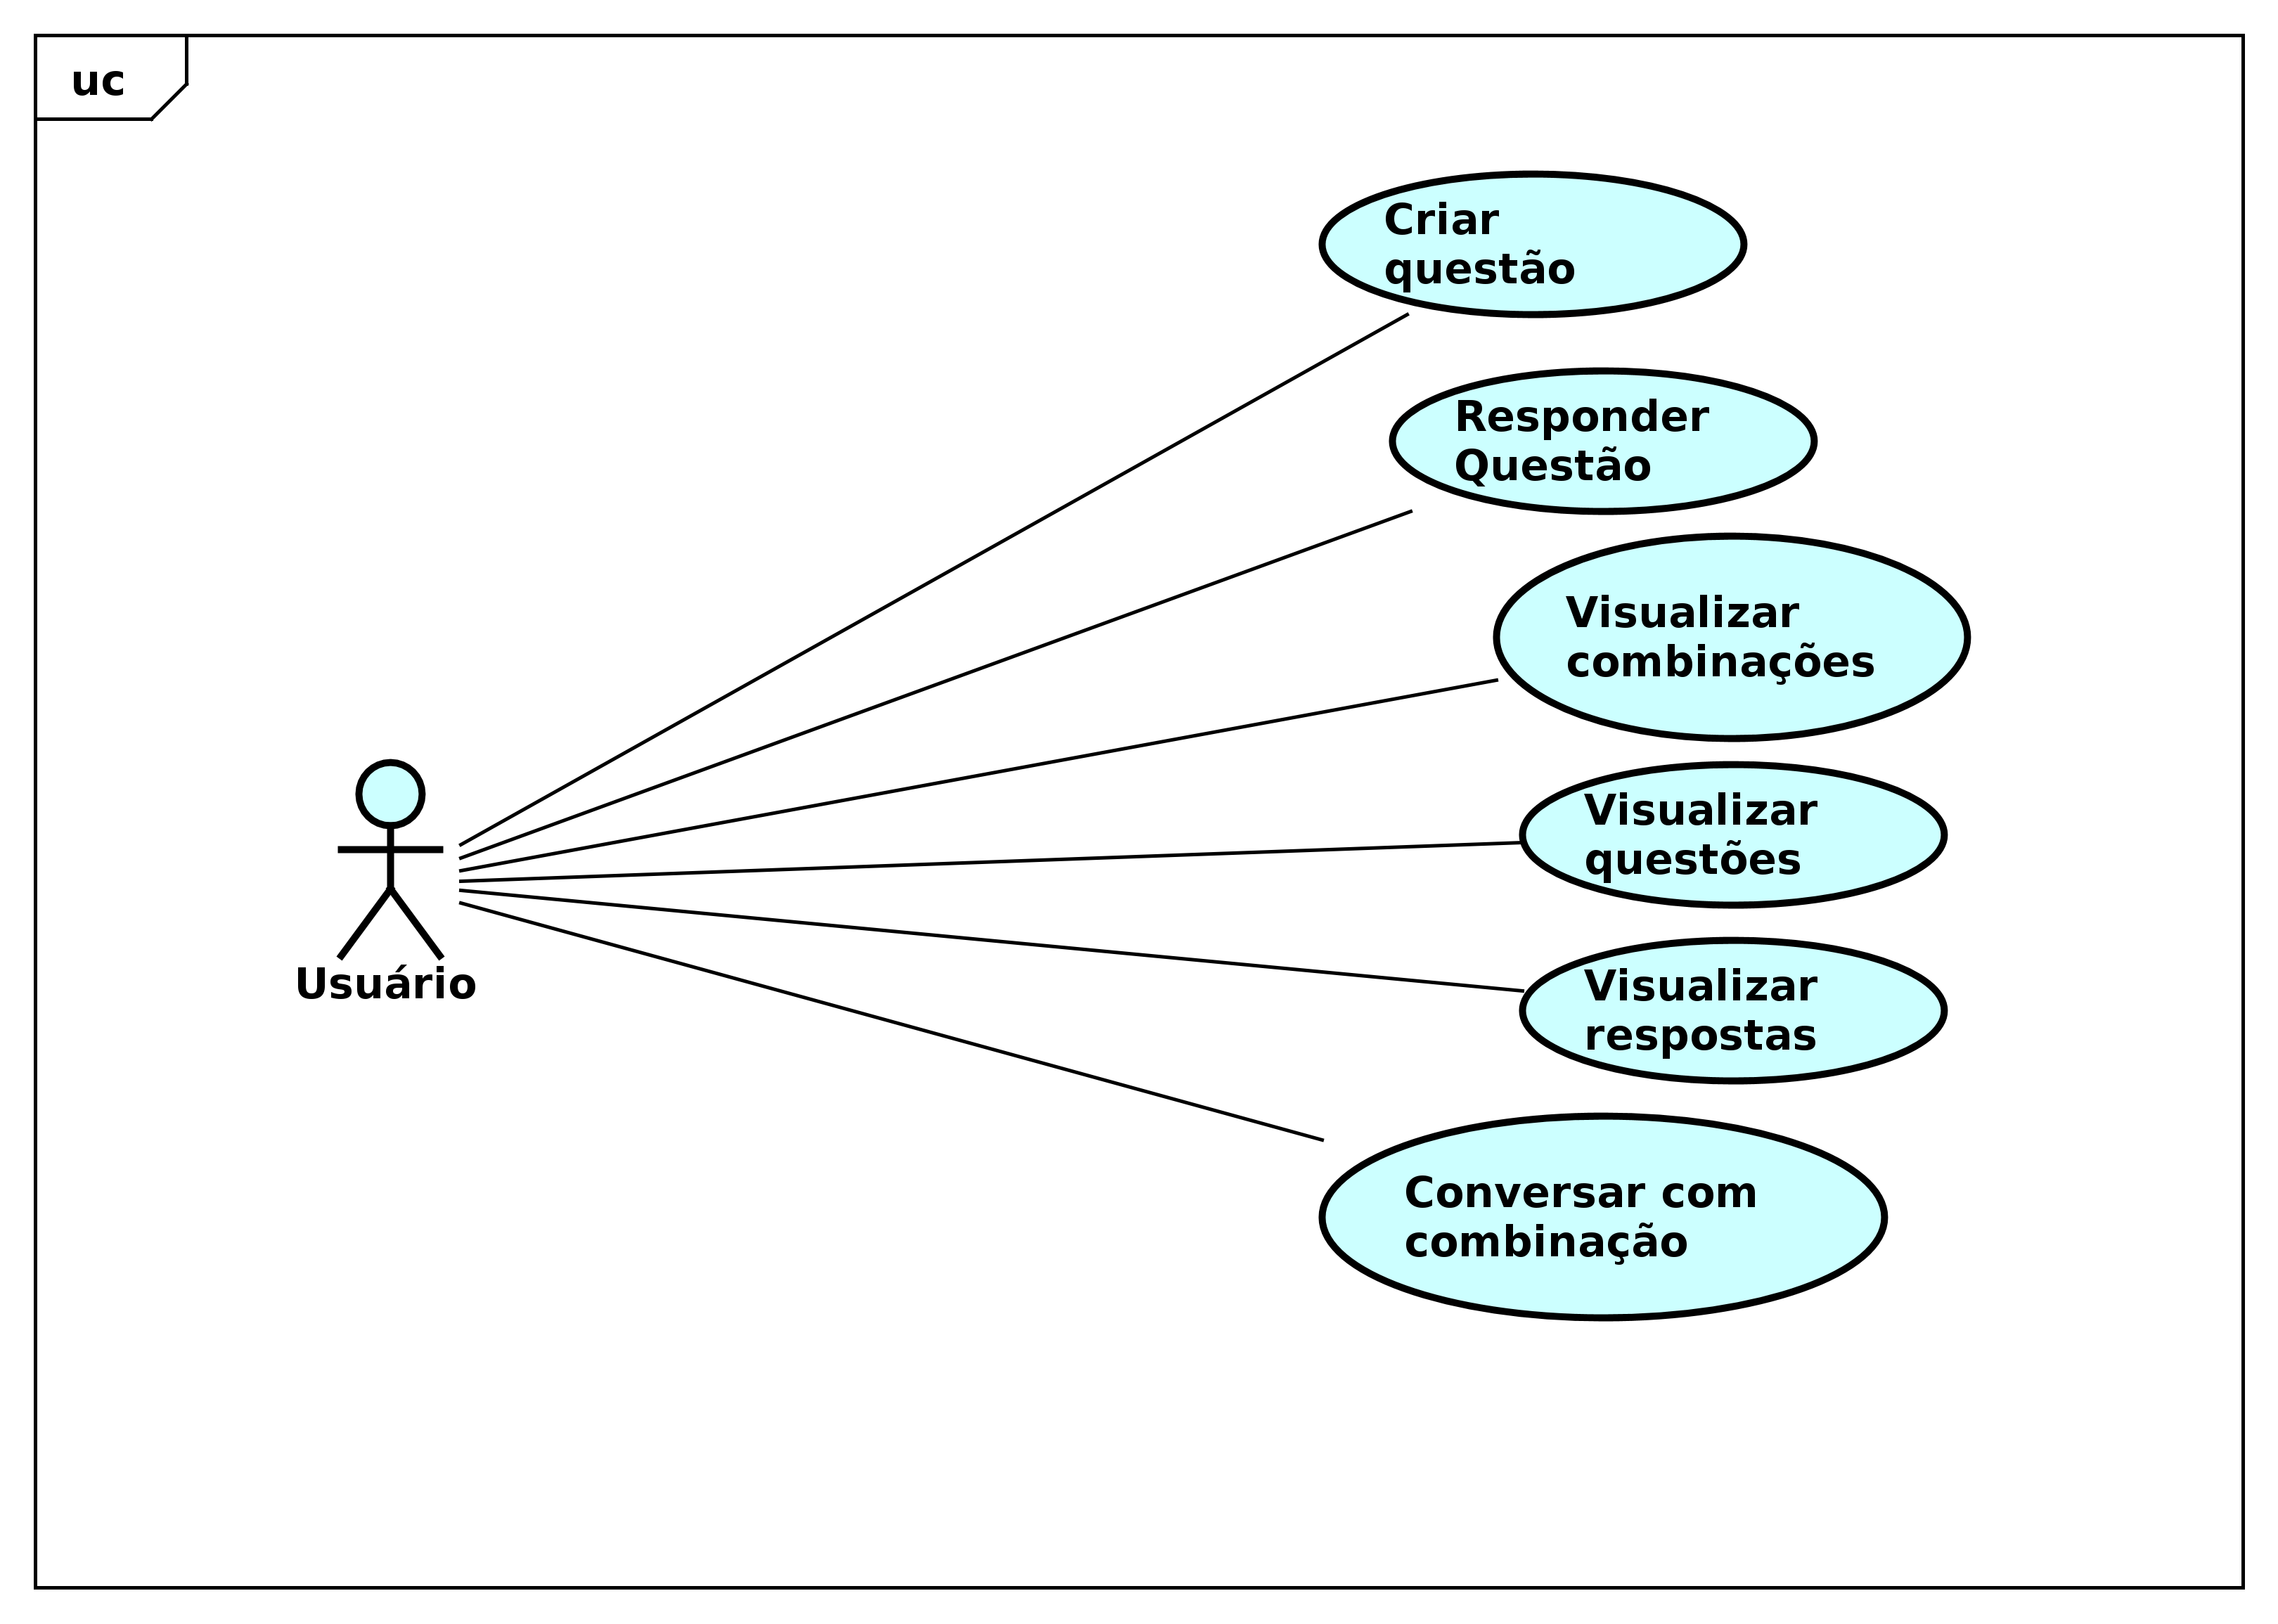
\includegraphics[width=16cm]{DCU1.png}
\caption{Diagrama de caso de uso nível 1. Fonte: os autores.}
\label{fig:DCU1}
\end{figure}

\begin{figure}[!htb]
\centering
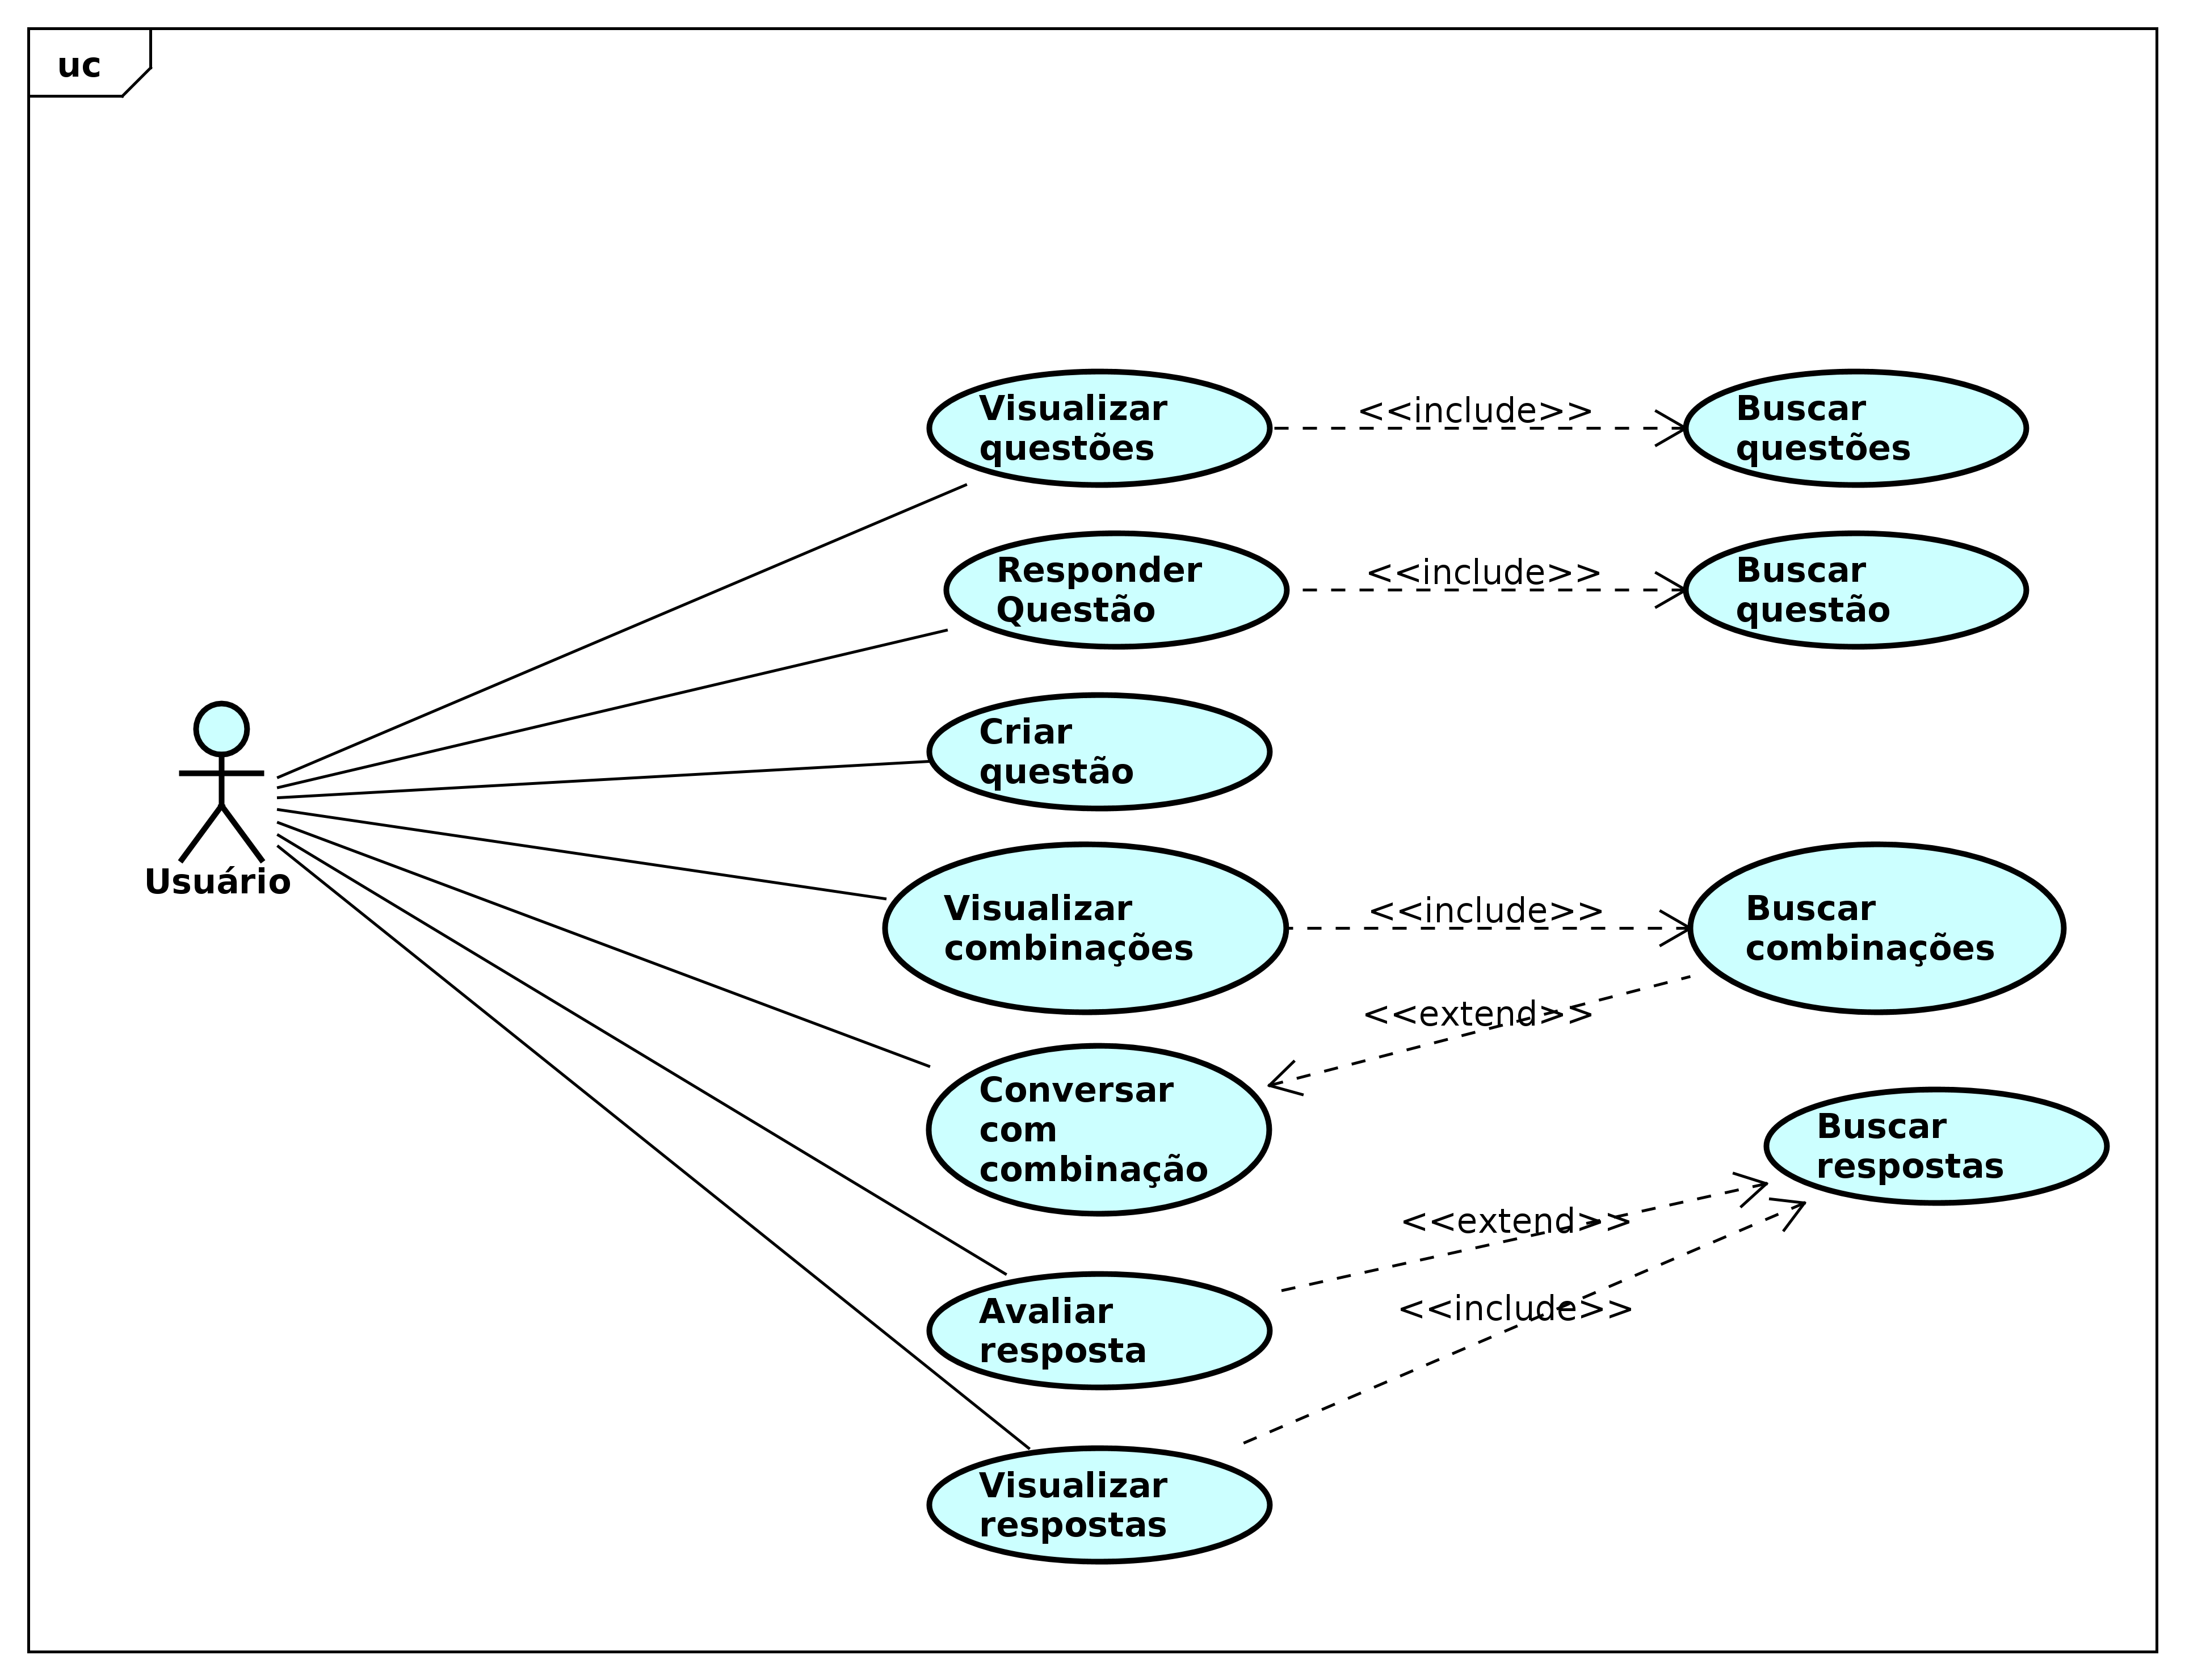
\includegraphics[width=16cm]{DCU2.png}
\caption{Diagrama de caso de uso nível 2. Fonte: os autores.}
\label{fig:DCU2}
\end{figure}
%=====================================================

Diagramas de sequência

\begin{figure}[!htb]
\centering
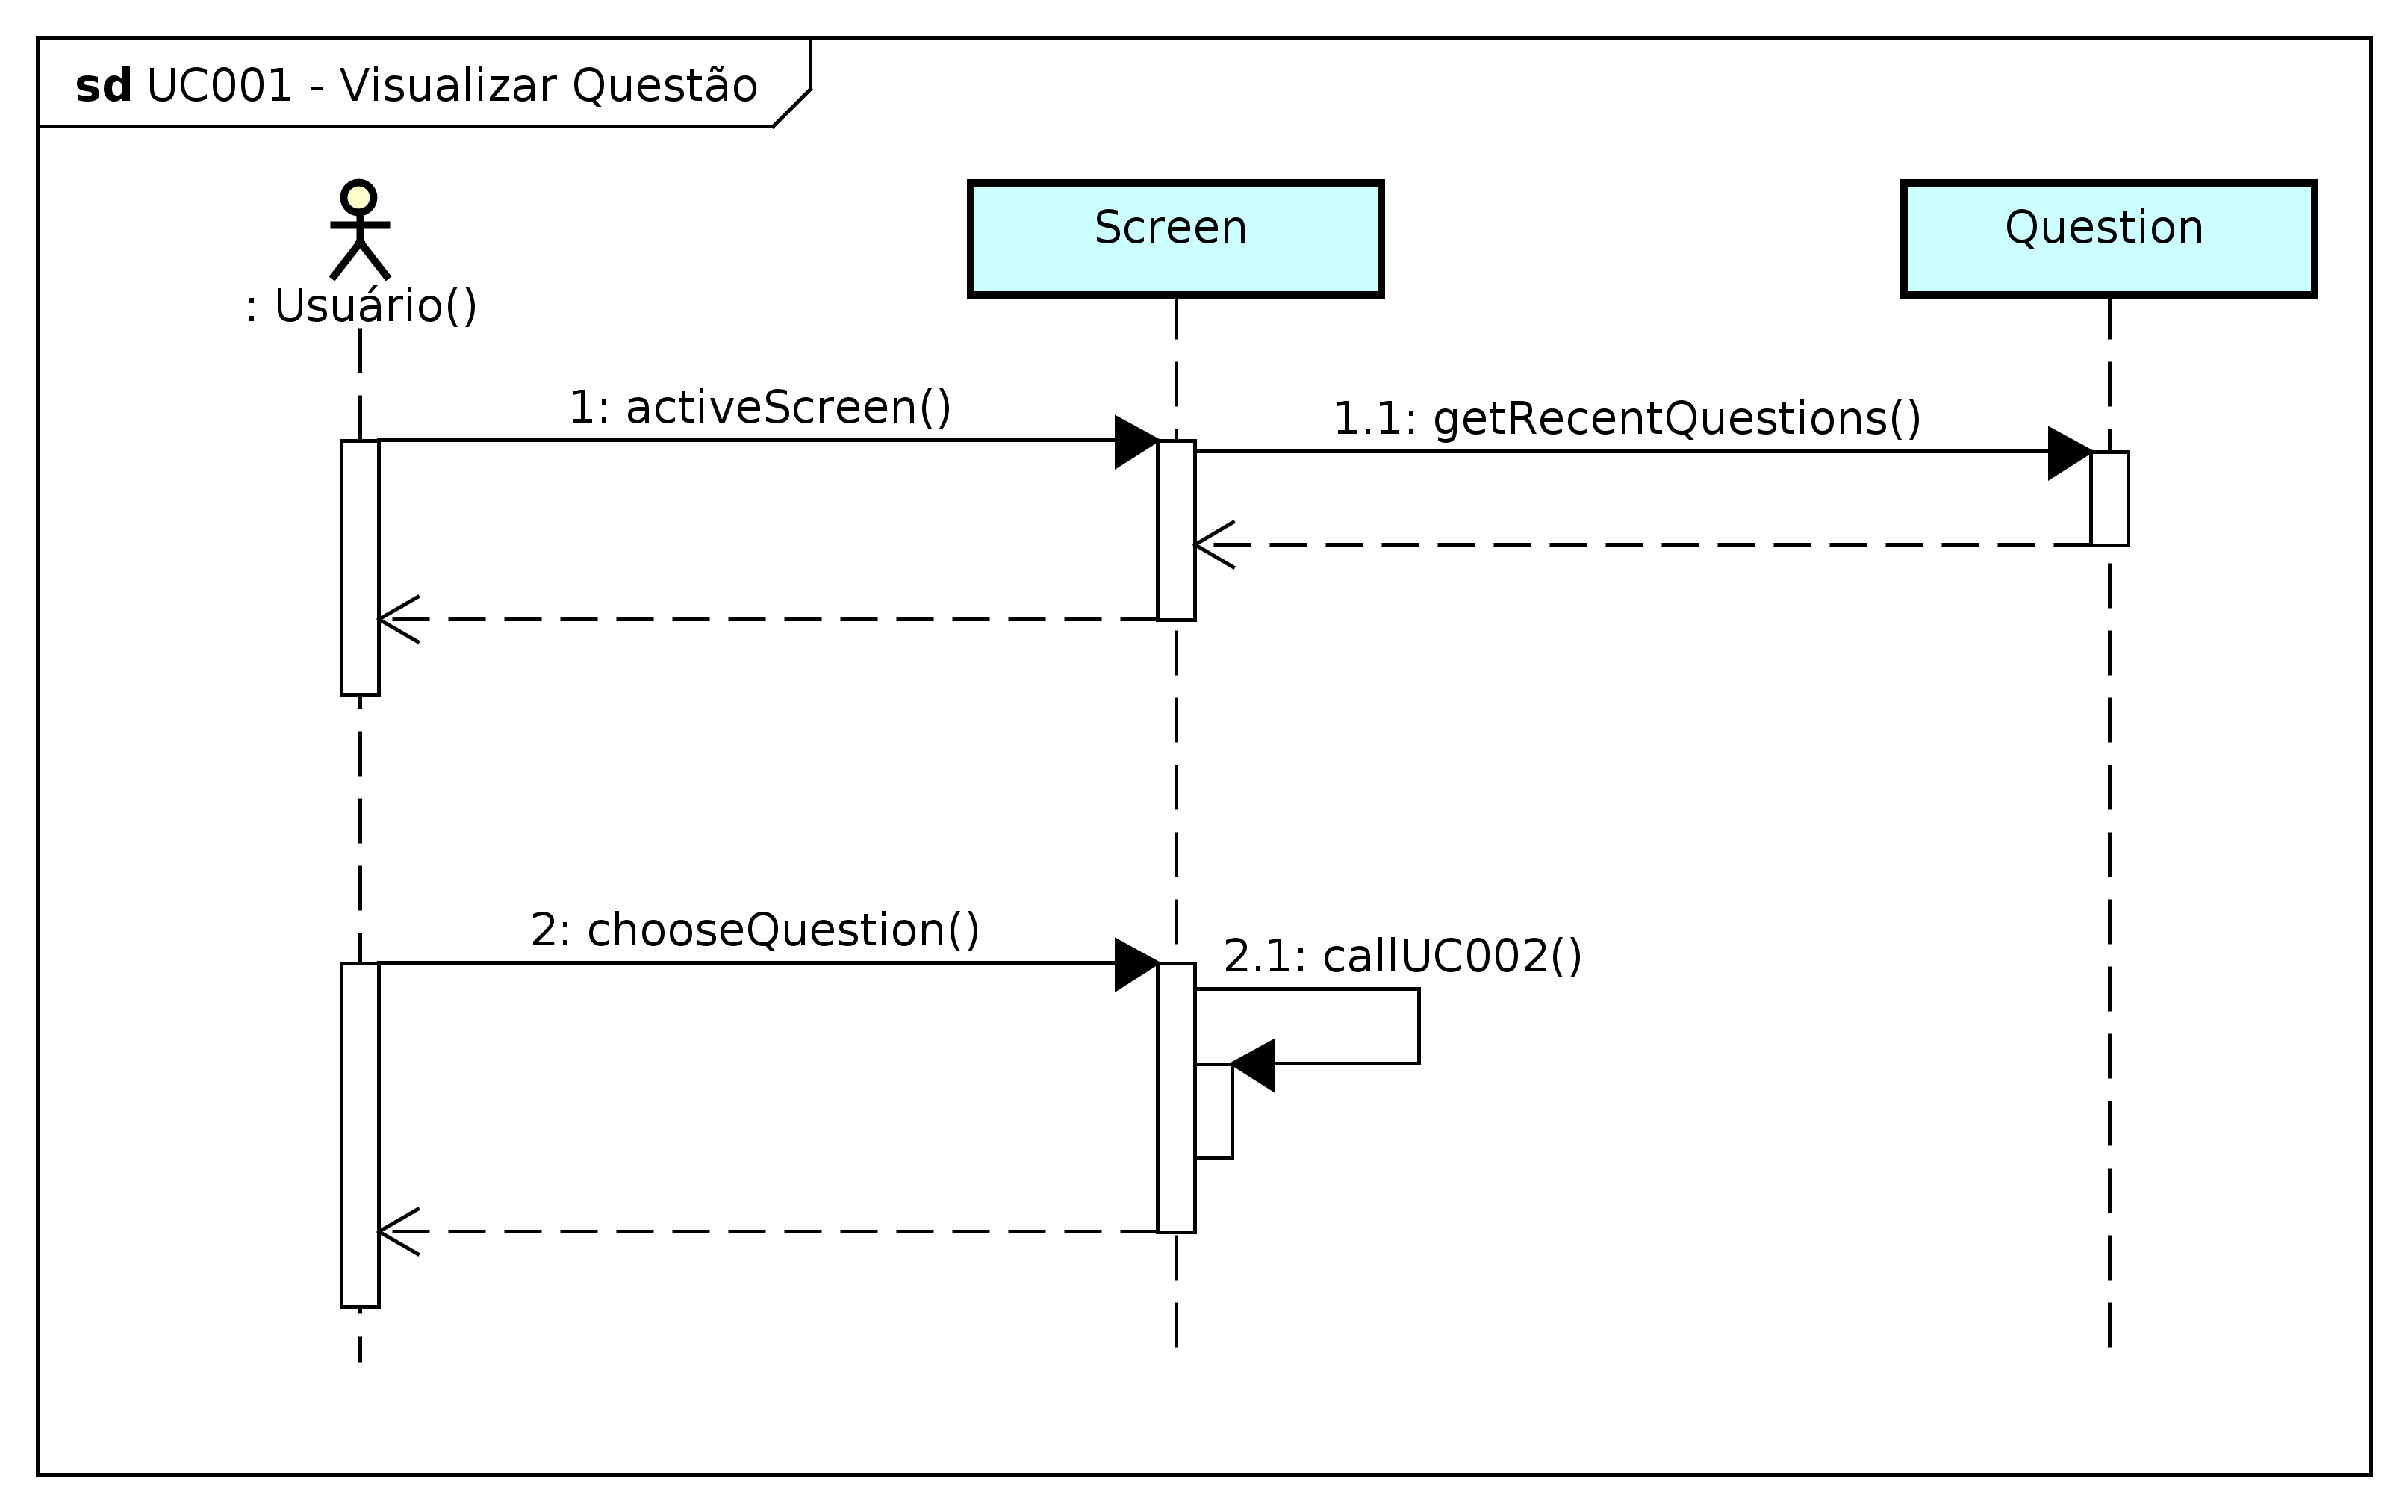
\includegraphics[width=16cm]{UC001-VisualizarQuestao.png}
\caption{Diagrama de caso de uso UC001 - Visualizar Questão. Fonte: os autores.}
\label{fig:UC001}
\end{figure}

\begin{figure}[!htb]
\centering
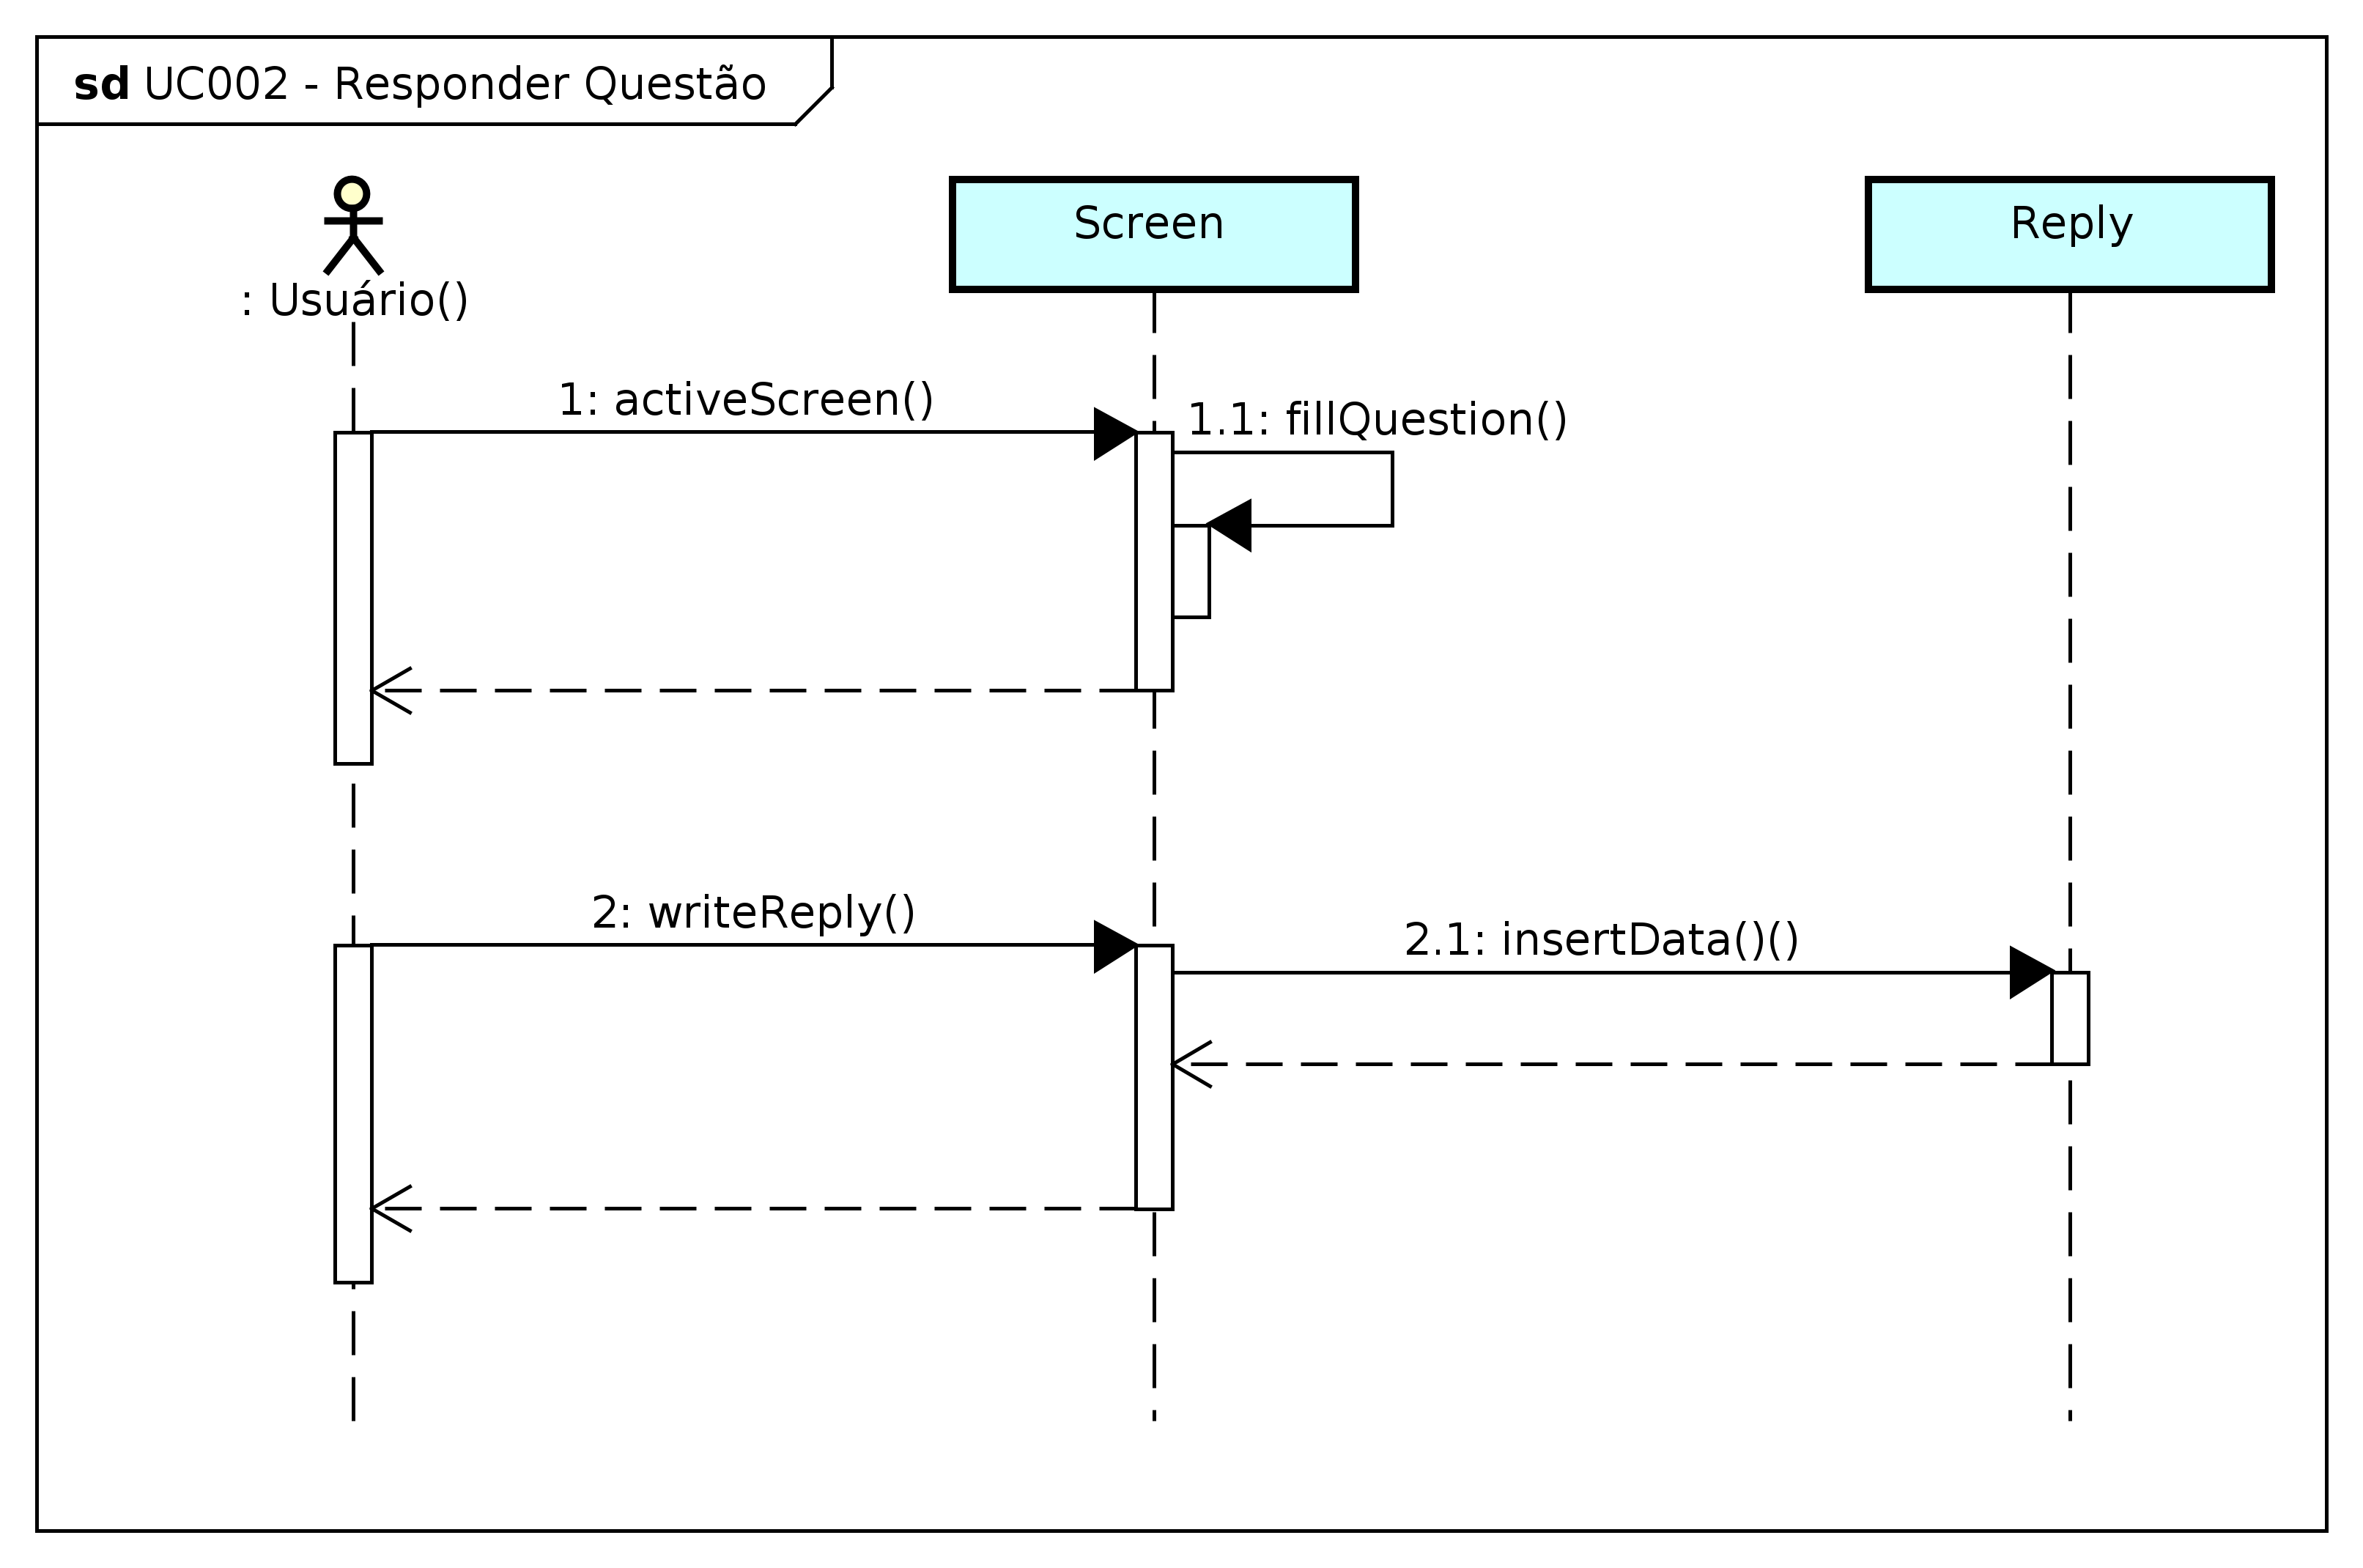
\includegraphics[width=16cm]{UC002-ResponderQuestao.png}
\caption{Diagrama de caso de uso UC002 - Responder Questão. Fonte: os autores.}
\label{fig:UC002}
\end{figure}

\begin{figure}[!htb]
\centering
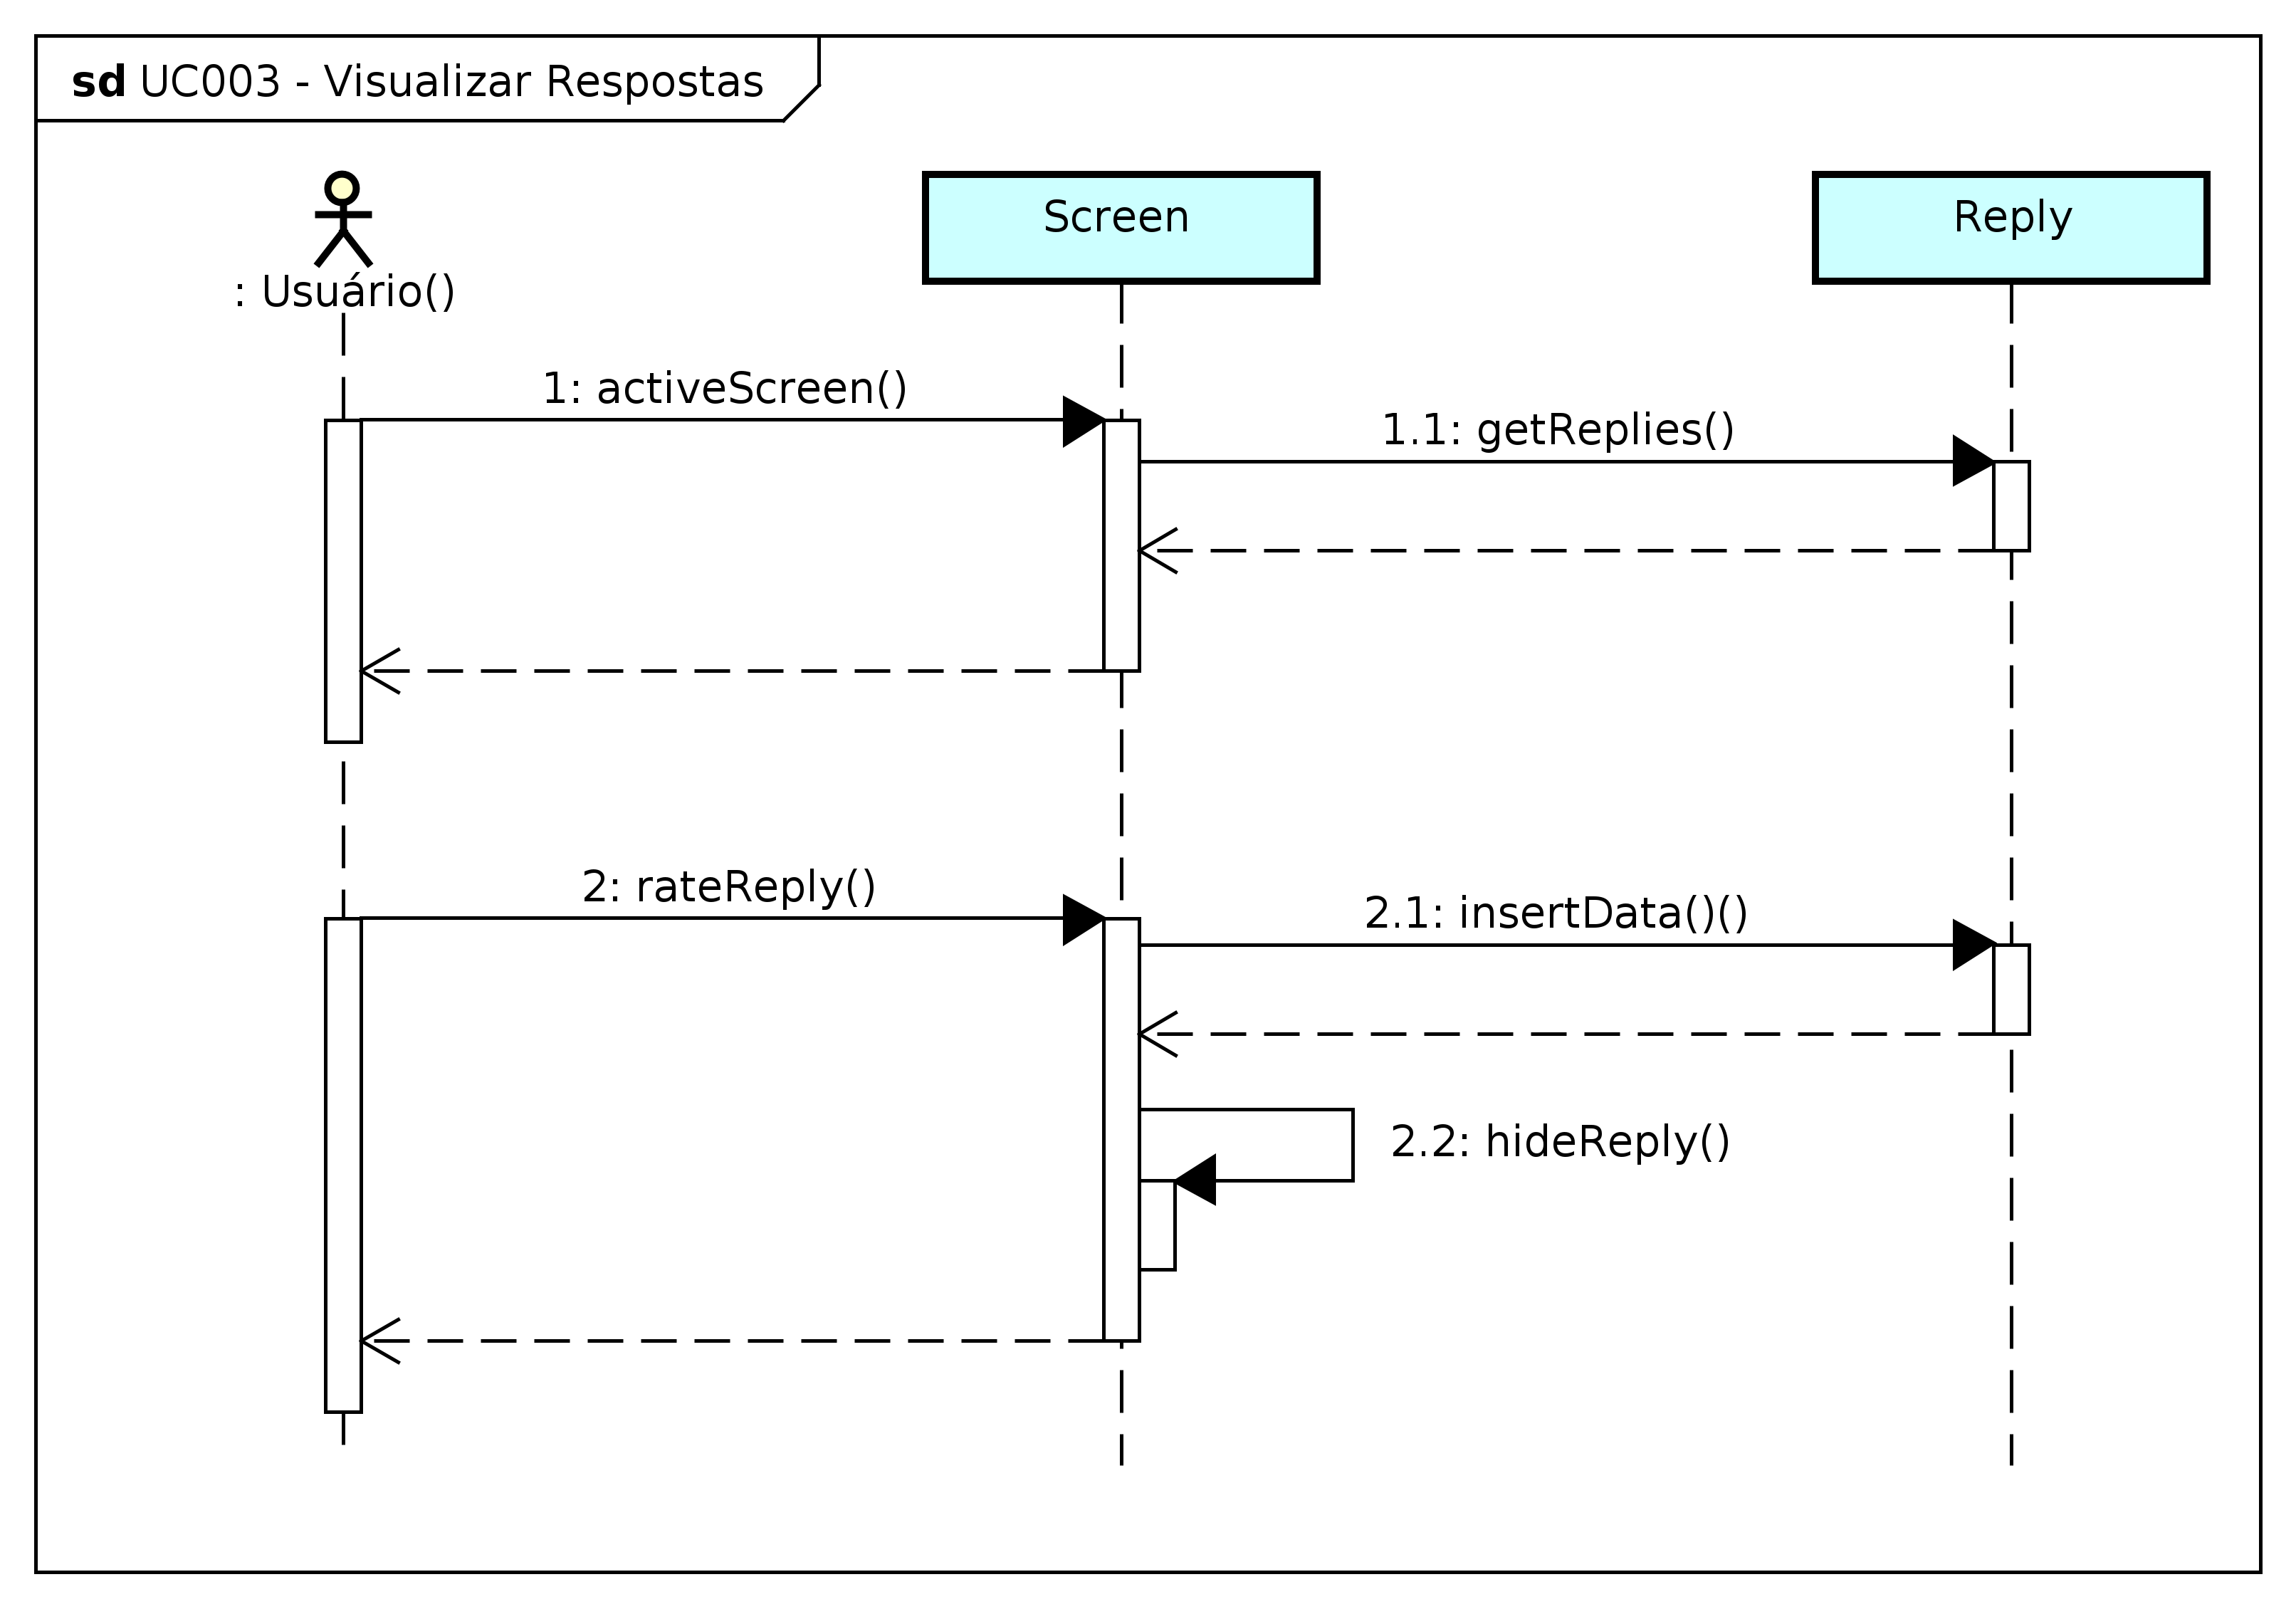
\includegraphics[width=16cm]{UC003-VisualizarRespostas.png}
\caption{Diagrama de caso de uso UC003 - Visualizar Respostas. Fonte: os autores.}
\label{fig:UC003}
\end{figure}


\begin{figure}[!htb]
\centering
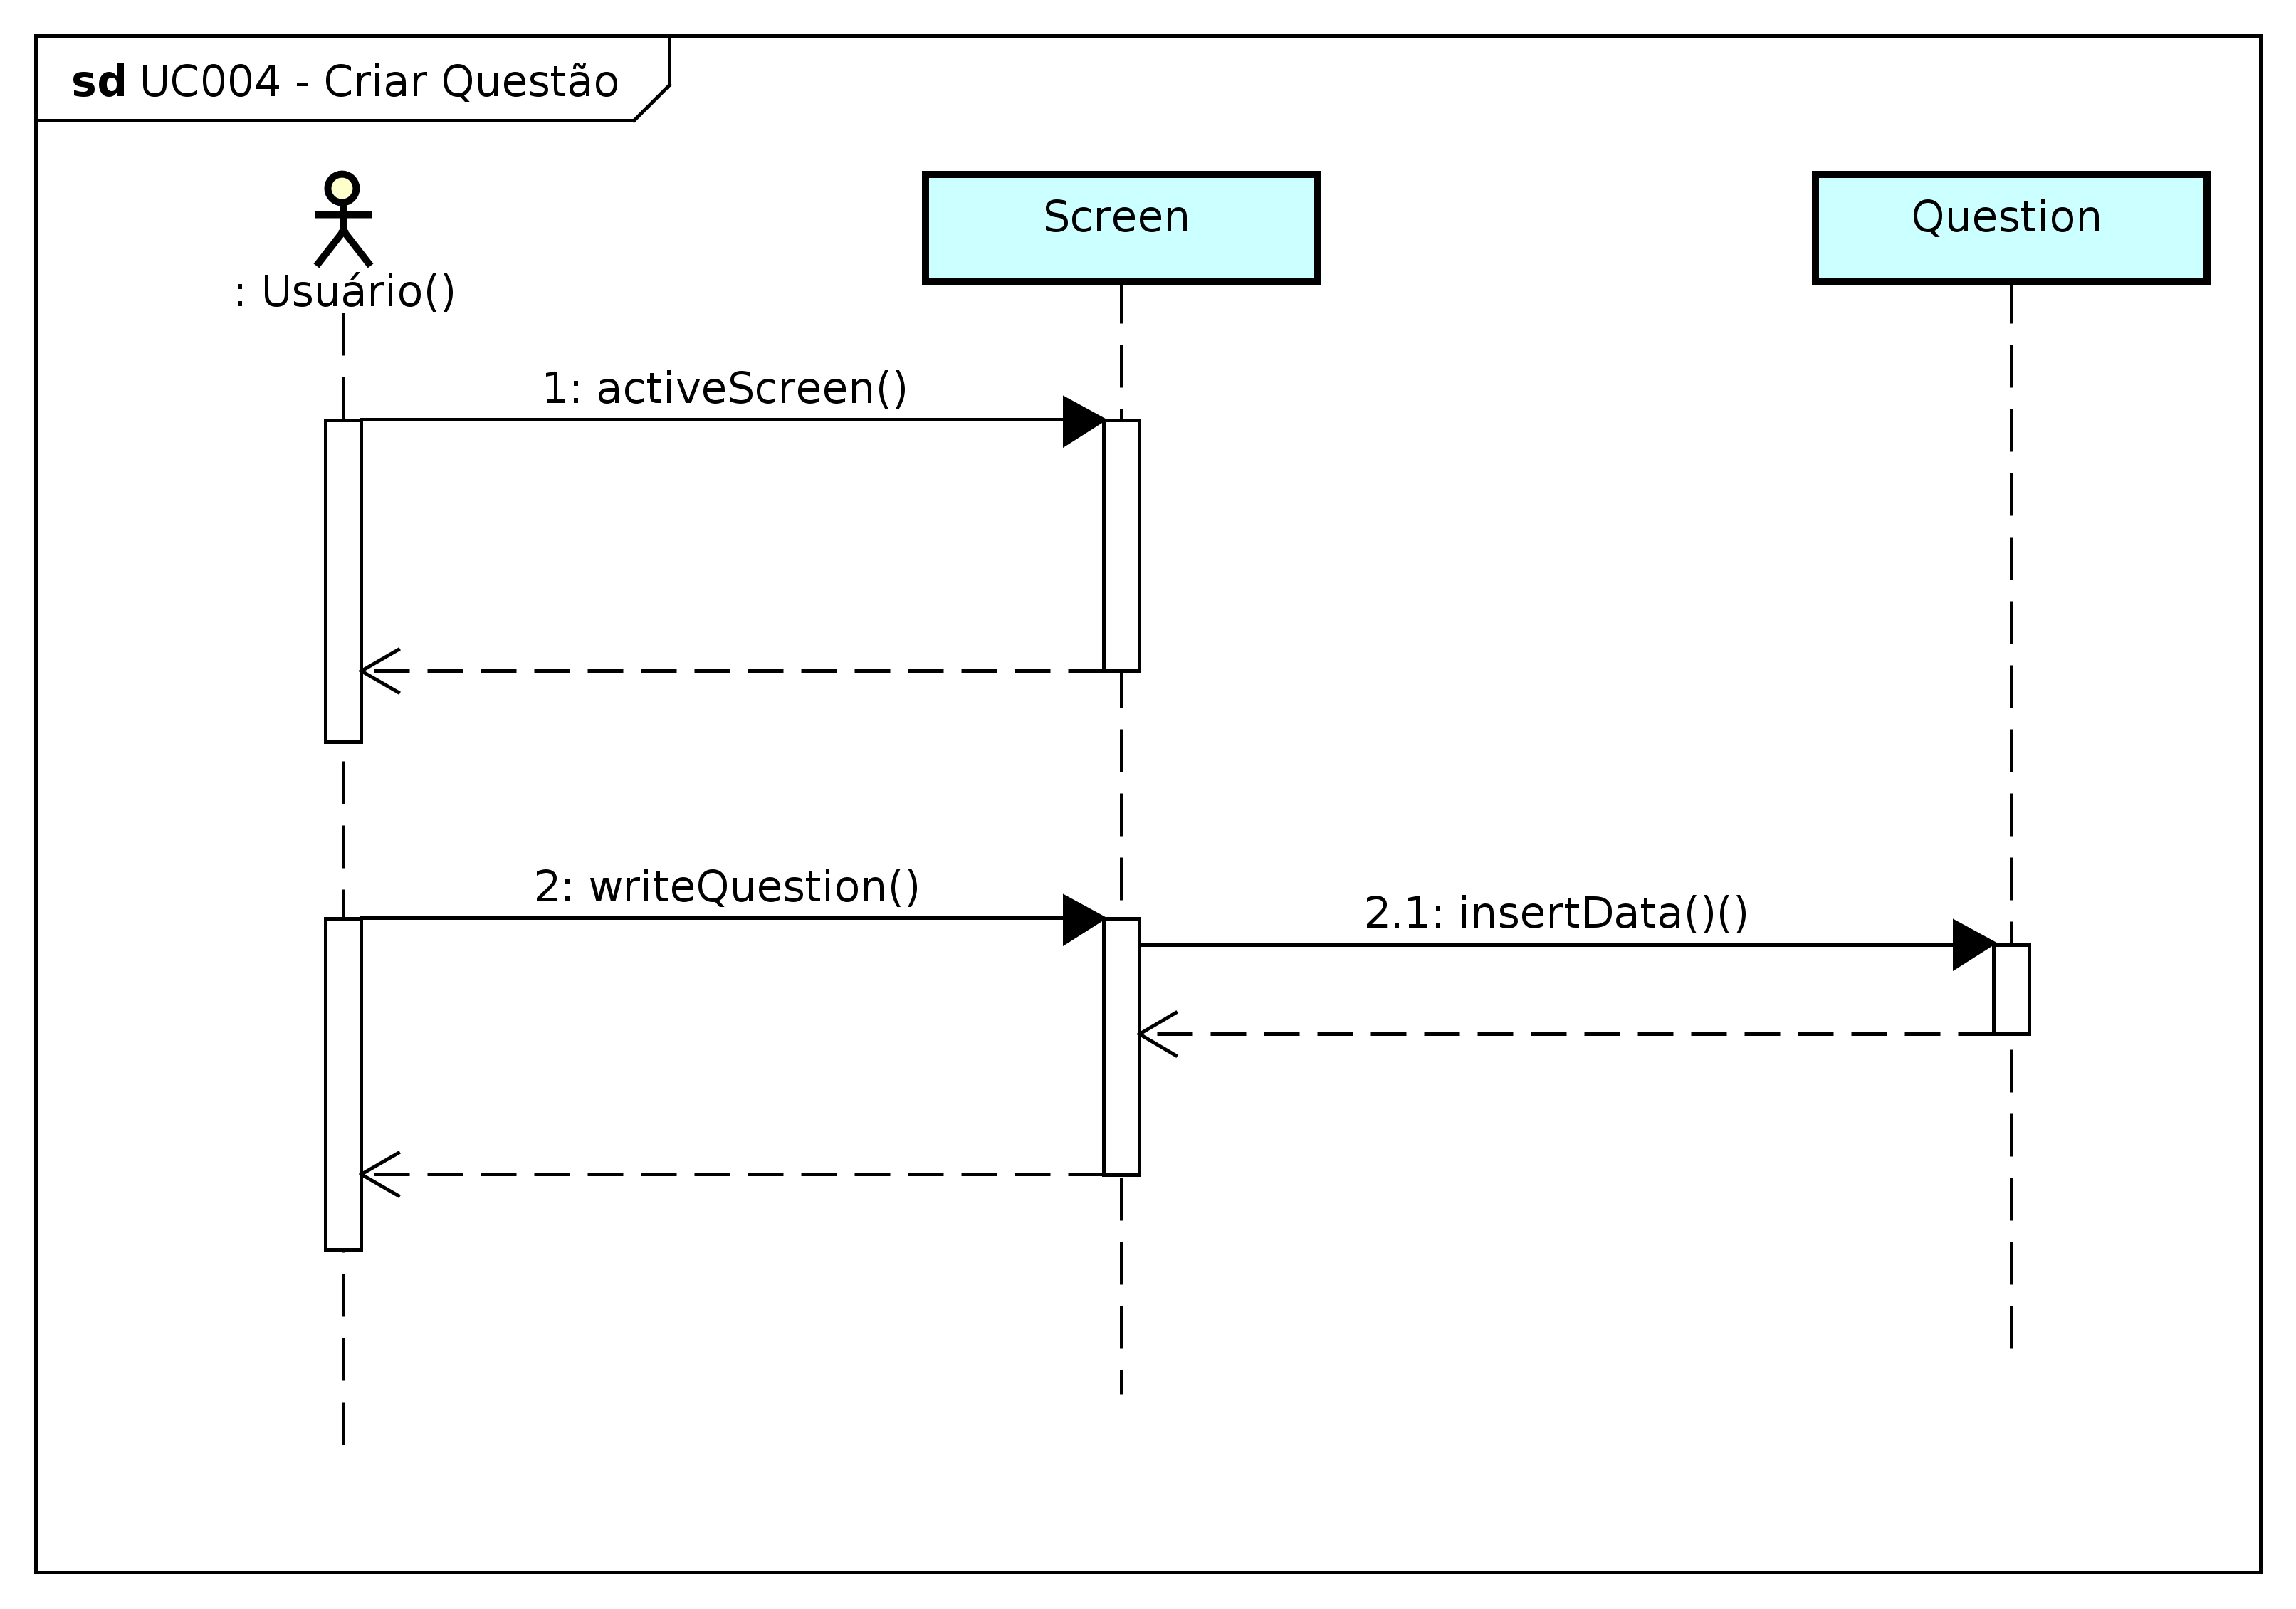
\includegraphics[width=16cm]{UC004-CriarQuestao.png}
\caption{Diagrama de caso de uso UC004 - Criar Questão. Fonte: os autores.}
\label{fig:UC004}
\end{figure}


\begin{figure}[!htb]
\centering
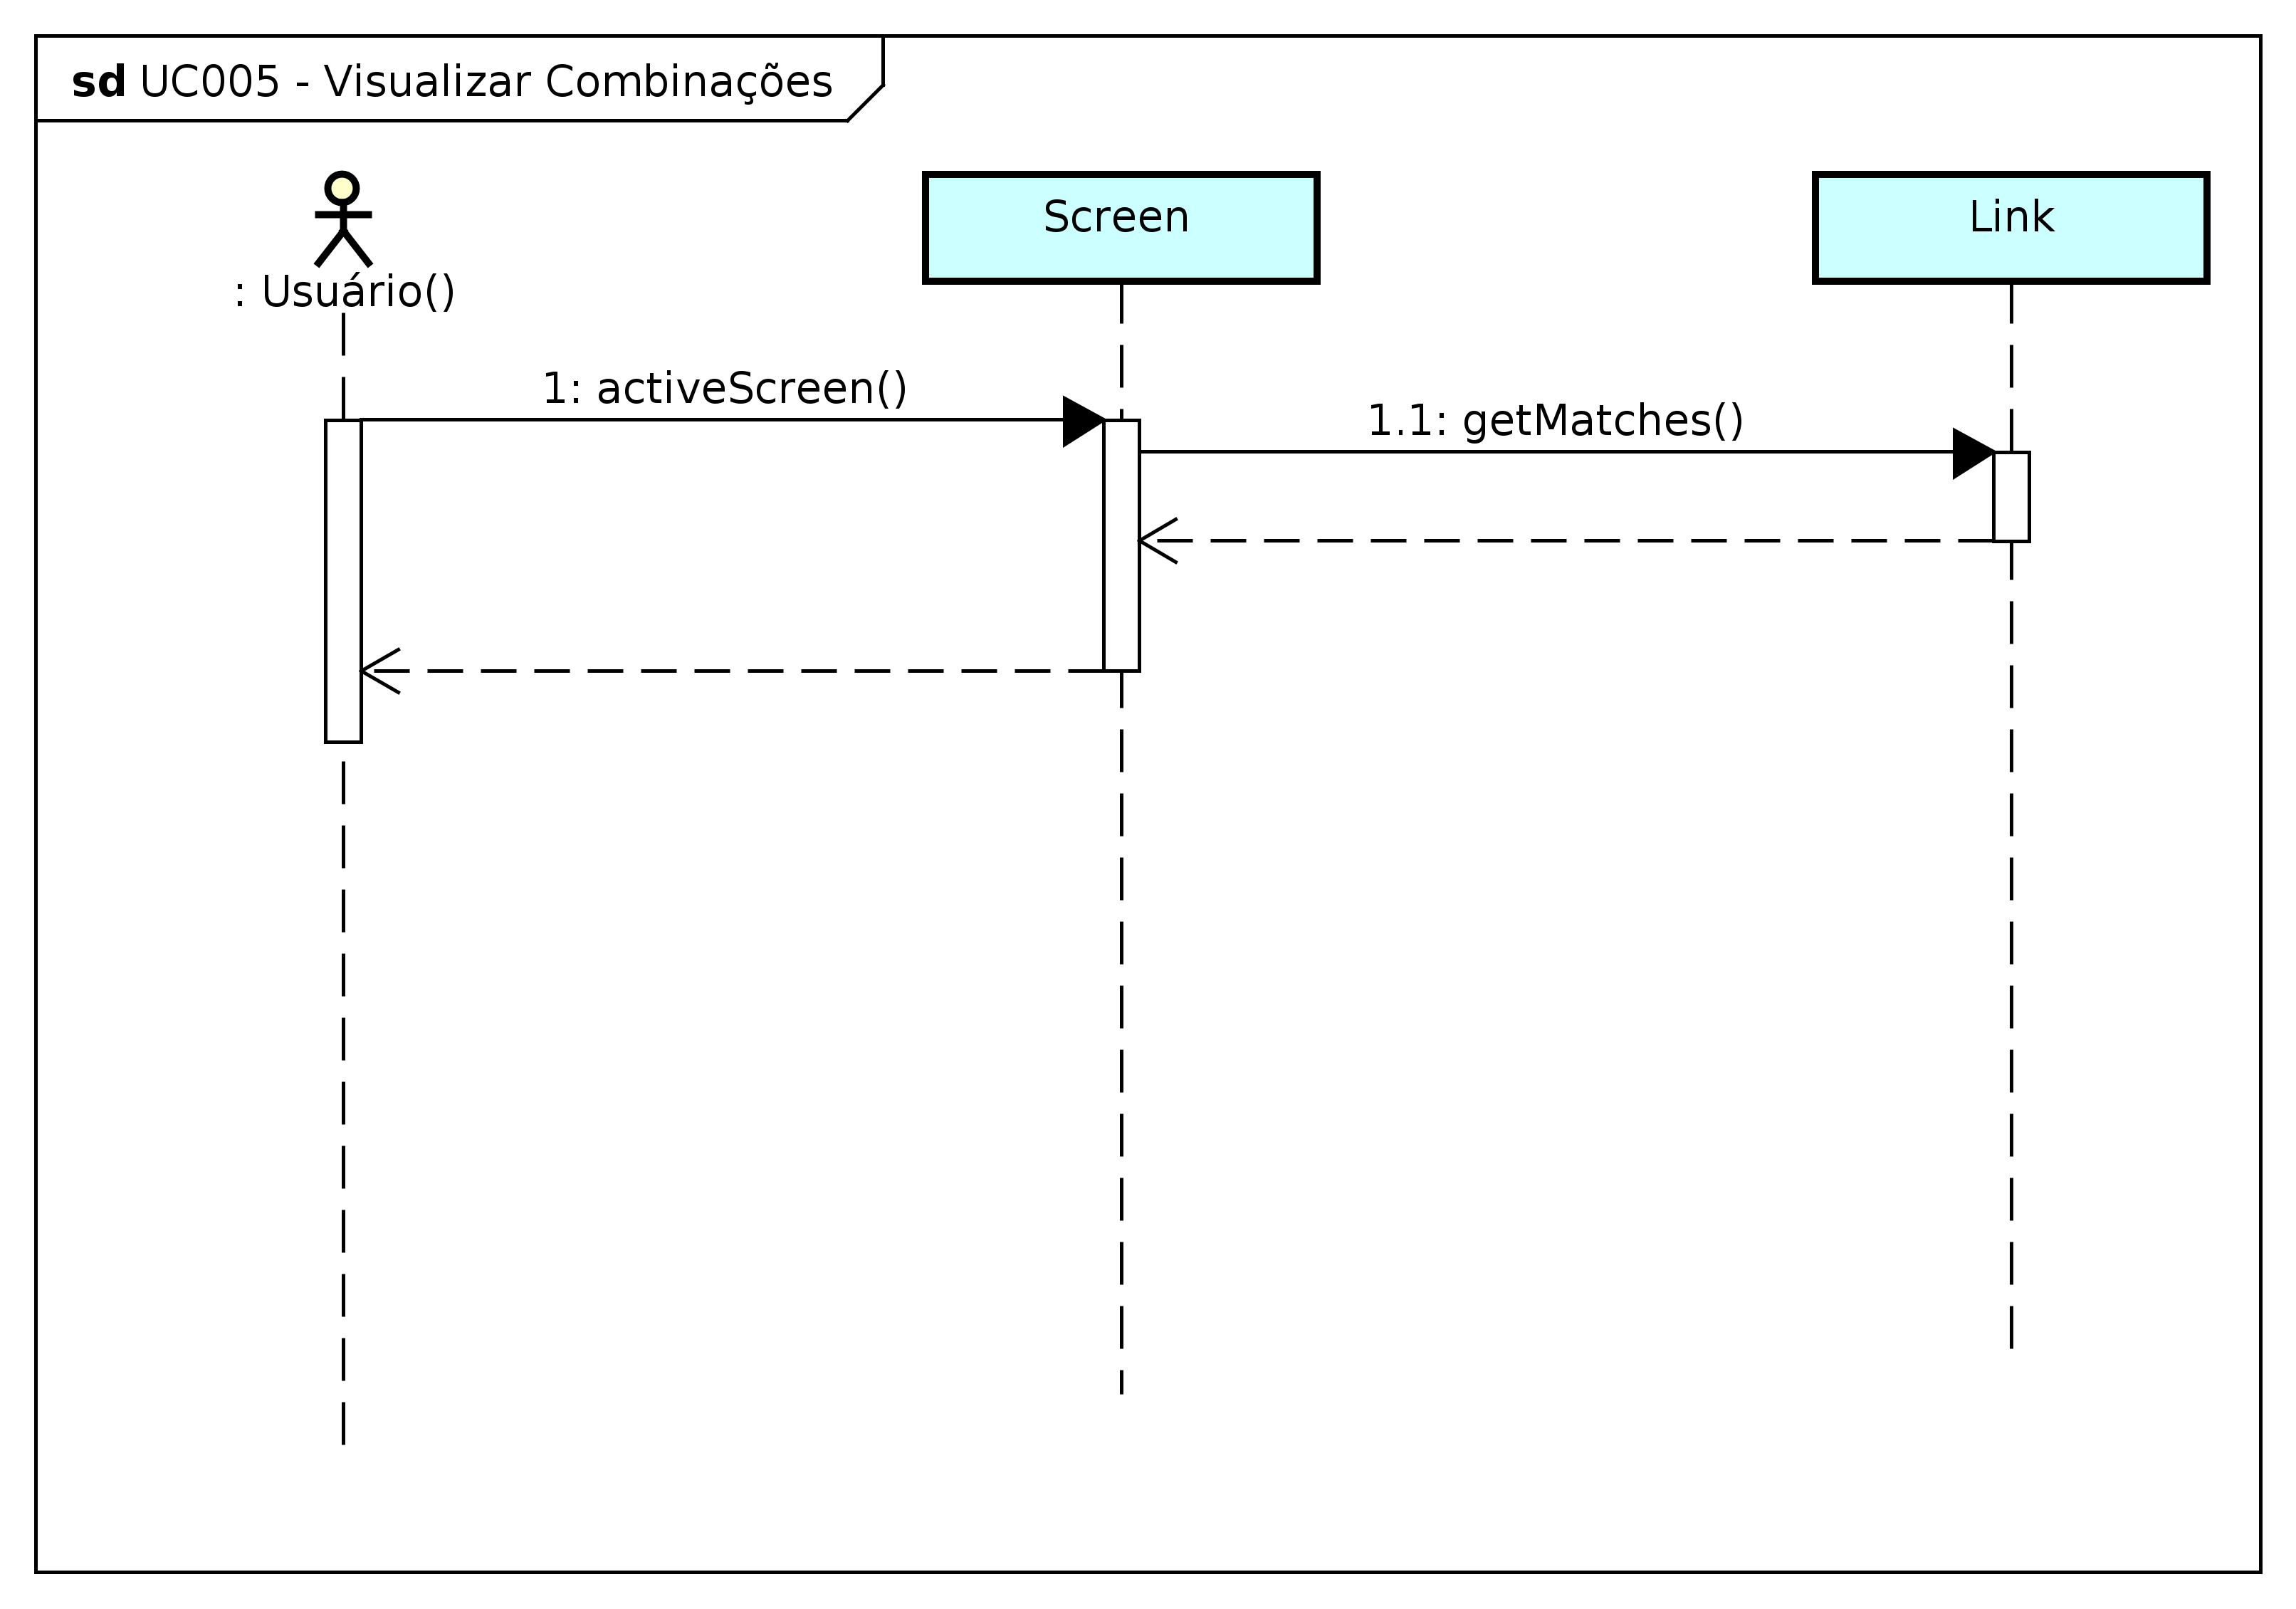
\includegraphics[width=16cm]{UC005-VisualizarCombinacoes.png}
\caption{Diagrama de caso de uso UC005 - Visualizar Combinações. Fonte: os autores.}
\label{fig:UC005}
\end{figure}


Diagrama de Classes

\begin{figure}[!htb]
\centering
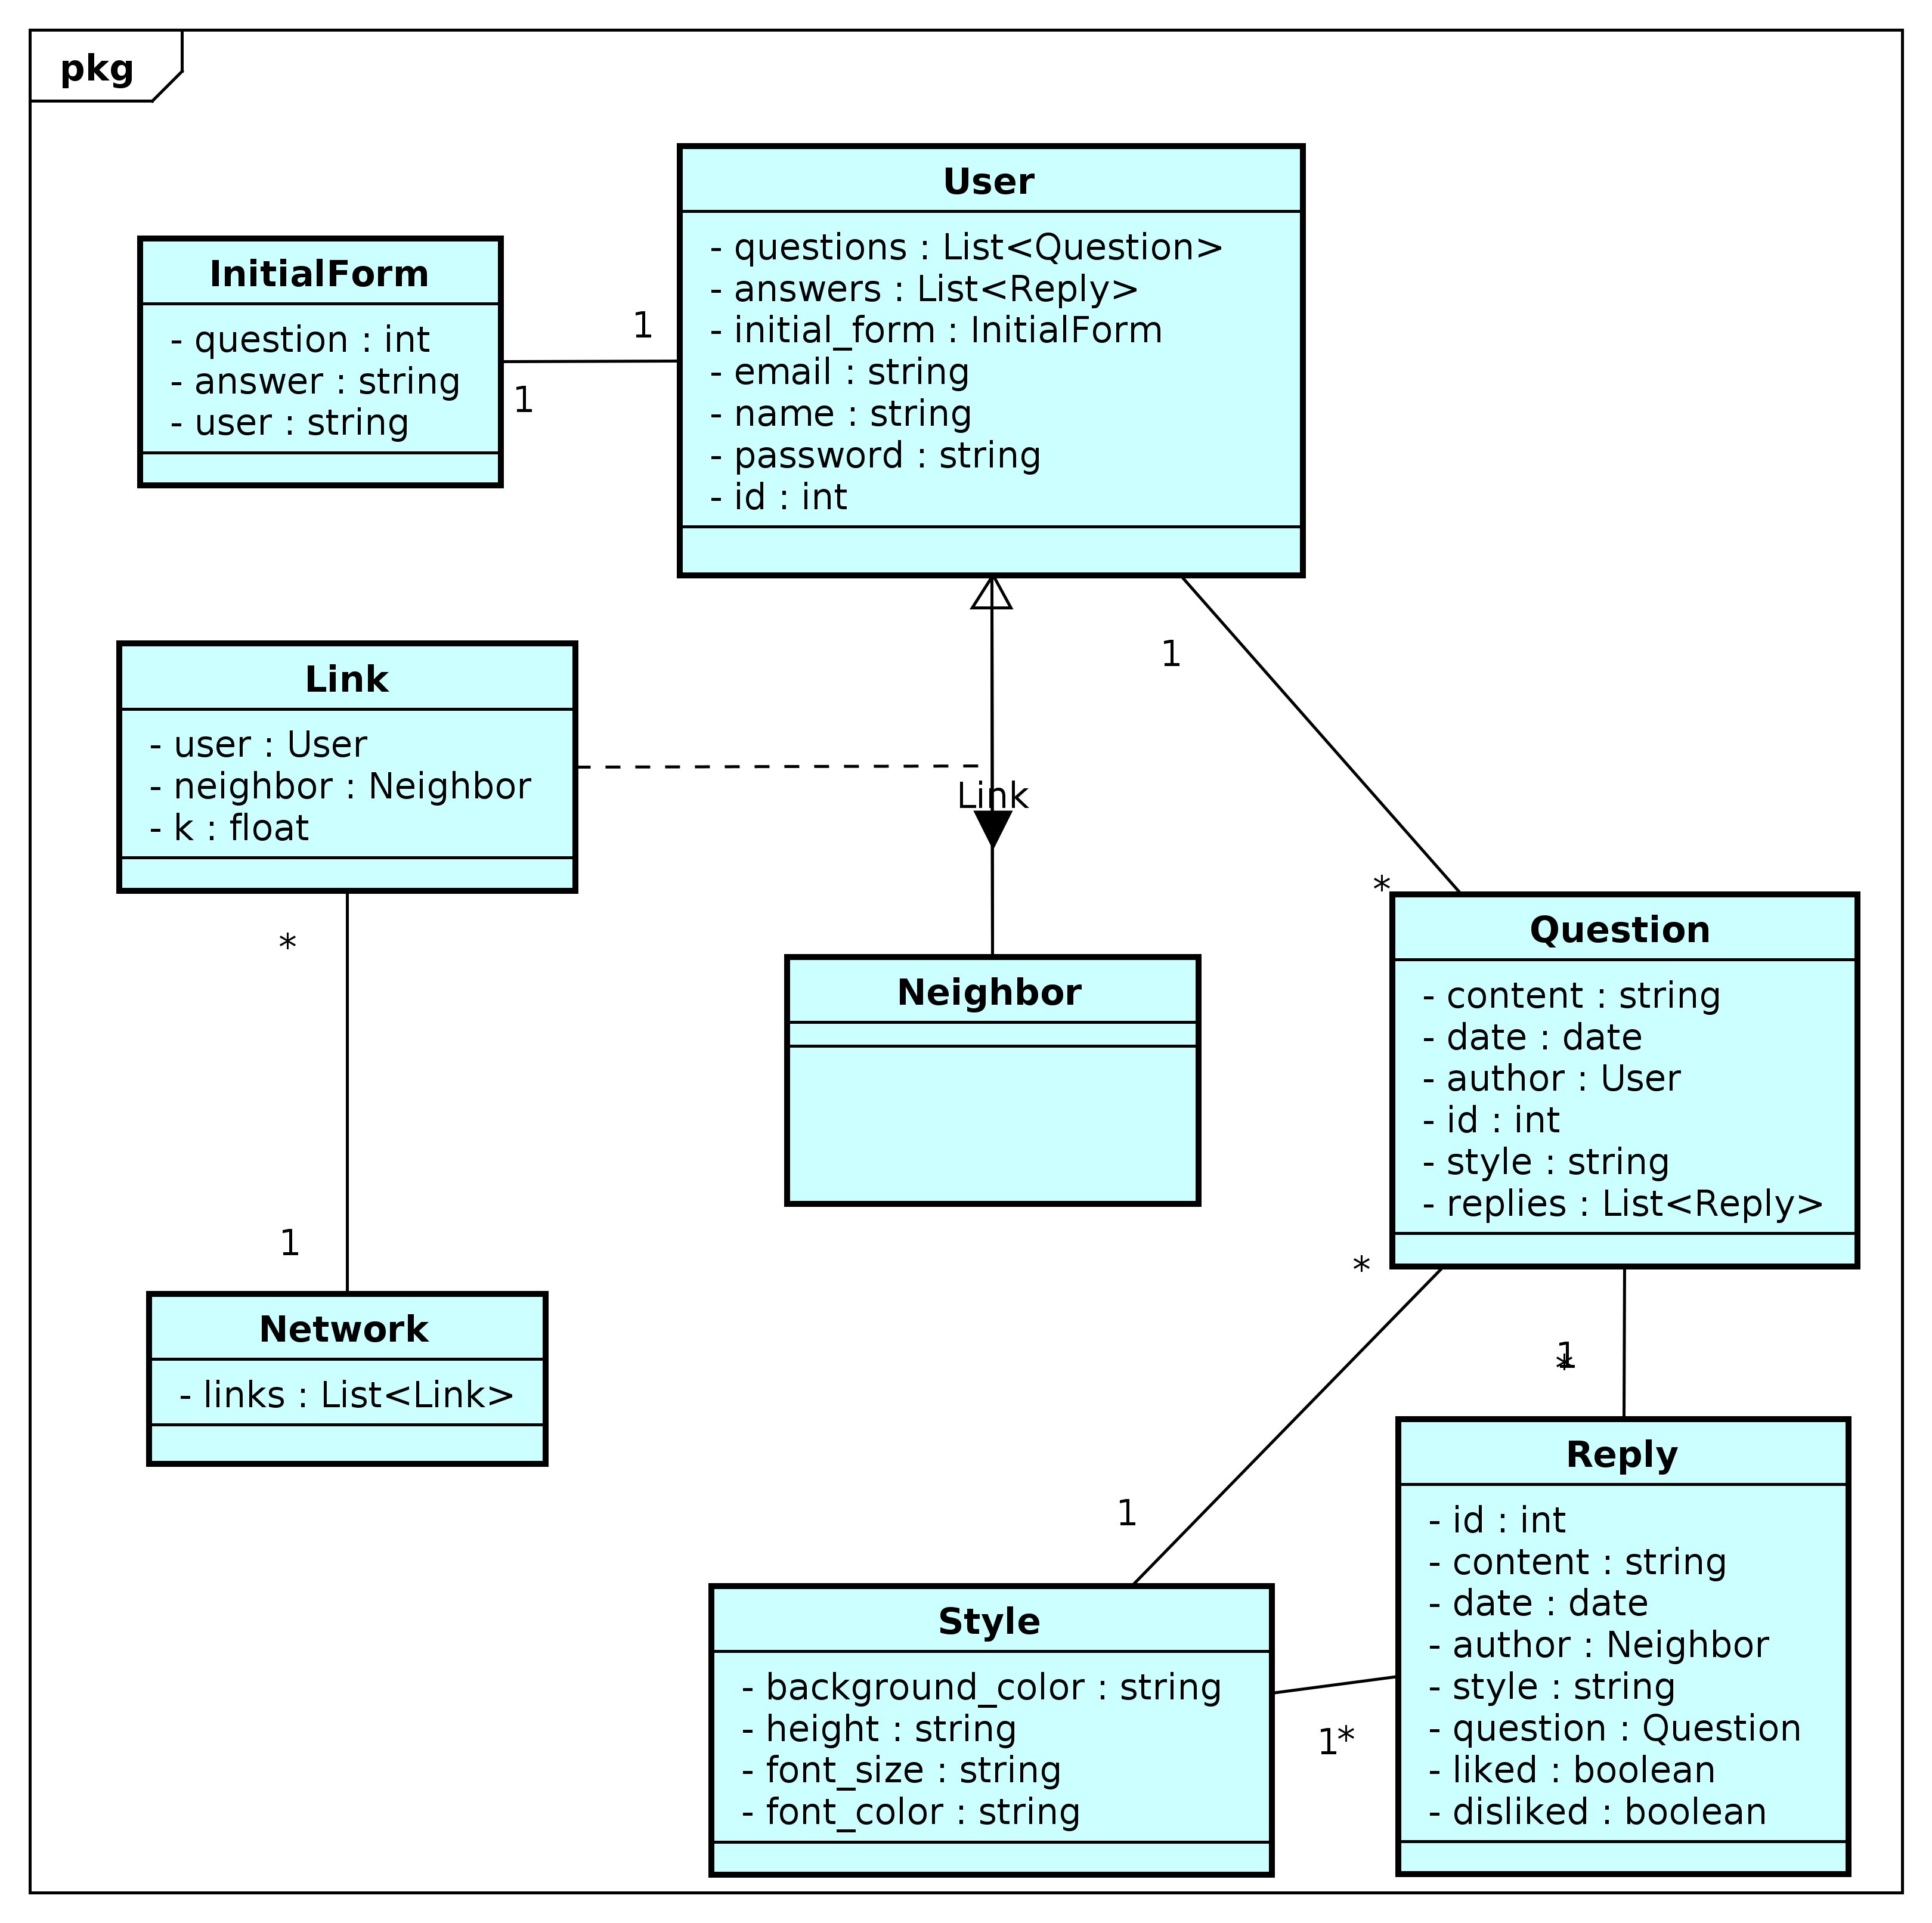
\includegraphics[width=16cm]{DiagramaClasse.png}
\caption{Diagrama de classes. Fonte: os autores.}
\label{fig:diagramaClasse}
\end{figure}
